\subsection{Упражнение 1}

Пилообразный сигнал линейно нарастает от -1 до 1, а затем резко падает до -1 и повторяется.

\noindent Напишите класс, называемый SawtoothSignal, расширяющий signal и предоставляющий evaluate для оценки пилообразного сигнала.

\noindent Вычислите спектр пилообразного сигнала. Как соотносится его гармоническая структура с тругольными с прямоугольными сигналами?

Создадим класс SawtoothSignal:

\begin{lstlisting}[language=Python]
import thinkdsp
class SawtoothSignal(thinkdsp.Sinusoid):
  def evaluate(self, ts):
    cycles = self.freq * ts + self.offset / np.pi / 2
    frac, _ = np.modf(cycles)
    ys = thinkdsp.normalize(thinkdsp.unbias(frac), self.amp)
    return ys
\end{lstlisting}

Сделаем пилообразный сигнал и вычислим спектр

\begin{lstlisting}[language=Python]
saw = SawtoothSignal()
saw.plot()
saw_wave = saw.make_wave(duration=1, framerate=10000)
decorate(xlabel='Time (s)')
\end{lstlisting}

\begin{figure}[H]
	\begin{center}
		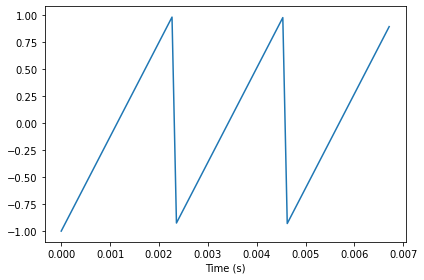
\includegraphics[scale=1]{fig/lab02/lab02_01.png}
		\caption{График пилообразного сигнала}
	\end{center}
\end{figure}

Вычислим спектр:

\begin{lstlisting}[language=Python]
spectr = saw_wave.make_spectrum()
spectr.plot()
decorate(xlabel='Frequency (Hz)')
\end{lstlisting}

\begin{figure}[H]
	\begin{center}
		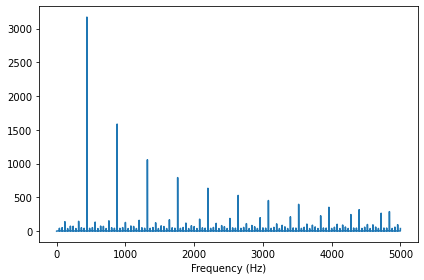
\includegraphics[scale=1]{fig/lab02/lab02_02.png}
		\caption{График спектра пилообразного сигнала}
	\end{center}
\end{figure}

Также, для сравнения, создадим прямоугольный и треугольный сигнал

\begin{lstlisting}[language=Python]
square = SquareSignal()
square.plot()
decorate(xlabel='Time (s)')
\end{lstlisting}

\begin{figure}[H]
	\begin{center}
		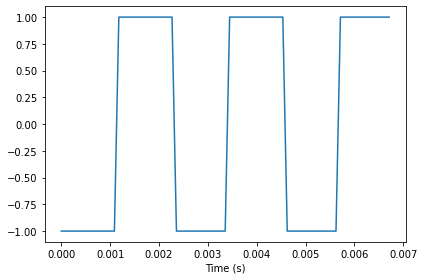
\includegraphics[scale=1]{fig/lab02/lab02_03.png}
		\caption{График прямоугольного сигнала}
	\end{center}
\end{figure}

\begin{lstlisting}[language=Python]
square.make_wave(duration=1, framerate=10000).make_spectrum().plot()
decorate(xlabel='Frequency (Hz)')
\end{lstlisting}

\begin{figure}[H]
	\begin{center}
		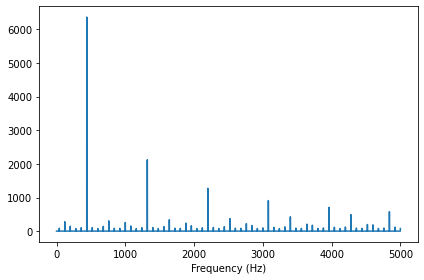
\includegraphics[scale=1]{fig/lab02/lab02_04.png}
		\caption{График спектра прямоугольного сигнала}
	\end{center}
\end{figure}


\begin{lstlisting}[language=Python]
tria = TriangleSignal()
tria.plot()
decorate(xlabel='Time (s)')
\end{lstlisting}

\begin{figure}[H]
	\begin{center}
		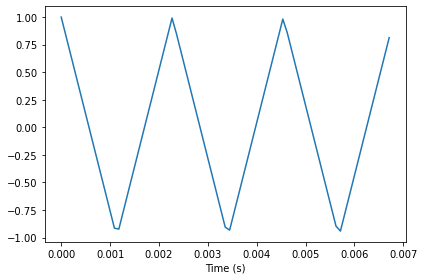
\includegraphics[scale=1]{fig/lab02/lab02_05.png}
		\caption{График треугольного сигнала}
	\end{center}
\end{figure}

\begin{lstlisting}[language=Python]
tria.make_wave(duration=1, framerate=10000).make_spectrum().plot()
decorate(xlabel='Frequency (Hz)')
\end{lstlisting}

\begin{figure}[H]
	\begin{center}
		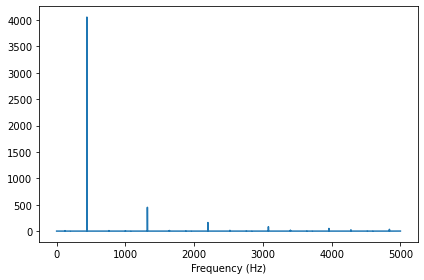
\includegraphics[scale=1]{fig/lab02/lab02_06.png}
		\caption{График спектра треугольного сигнала}
	\end{center}
\end{figure}

У треугольного сигнала нечетный гармоники, а амплитуда спадает пропорцинально квадрату частоты. У прямоугольного сигнала тоже только нечетный гармоники, спад по амплитуде пропорционален частоте. Пилообраный же сигнал падает пропорционально частоте и имеет как четные, так и нечетные гармоники.


\subsection{Упражнение 2}

Создайте прямоугольный сигнал 1100 Гц и вычислите wave с выборками 10 000 кадров в секунду. Постройте спектр и убедитесь, что большинство гармоник "завёрнуты" из-за биений, слышно ли последствия этого при проигрывании?

Создадим прямоугольный сигнал с частотой 1100Гц

\begin{lstlisting}[language=Python]
square = SquareSignal(1100)
sq_wave = square.make_wave(1, 0, 10000)
sq_wave.make_spectrum().plot()
decorate(xlabel='Frequency (Hz)')
\end{lstlisting}

\begin{figure}[H]
	\begin{center}
		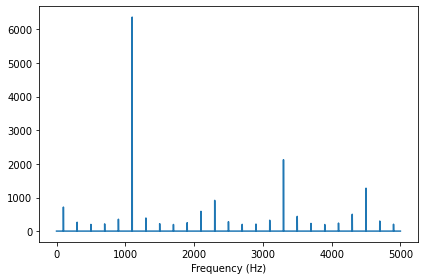
\includegraphics[scale=1]{fig/lab02/lab02_07.png}
		\caption{График прямоугольного сигнала с частотой 1100 Hz}
	\end{center}
\end{figure}

Видим заернутось гармоний из-за биения
\begin{lstlisting}[language=Python]
sq_wave.make_audio()
\end{lstlisting}


\subsection{Упражнение 3}

Возьмите объект спектра spectrum, и выведите первые несколько значений spectrum.fs, вы увидите, что частоты начинаются с нуля. Итак, «spectrum.hs[0]» — это величина компонента с частотой 0. Но что это значит?

\noindent Попробуйте этот эксперимент:

1. Сделать треугольный сигнал с частотой 440 и создать Волну длительностью 0,01 секунды. Постройте форму волны.

2. Создайте объект Spectrum и напечатайте spectrum.hs[0]. Каковы амплитуда и фаза этой составляющей?

3. Установите spectrum.hs[0] = 100. Создайте волну из модифицированного спектра и выведите ее. Как эта операция влияет на форму сигнала?

Создадим треугольный сигнал, возьмем спектр и распечатаем значения spectrum.fs

\begin{lstlisting}[language=Python]
tr = TriangleSignal(440)
tr_wave = tr.make_wave(duration=0.01)
tr_wave.plot()
decorate(xlabel='Time (s)')
\end{lstlisting}

\begin{figure}[H]
	\begin{center}
		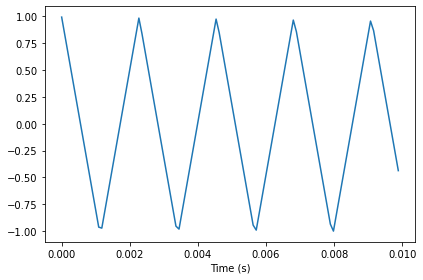
\includegraphics[scale=1]{fig/lab02/lab02_08.png}
		\caption{График треугольного сигнала с частотой 440 Hz}
	\end{center}
\end{figure}

Убедимся, что нулевой элемент равен 0

\begin{lstlisting}[language=Python]
tr_sp = tr_wave.make_spectrum()
tr_sp.hs[0]

(1.0436096431476471e-14+0j)
\end{lstlisting}

Изменим его на значение 100

\begin{lstlisting}[language=Python]
tr_sp.hs[0] = 100
tr_sp.make_wave().plot()
decorate(xlabel='Time (s)')
\end{lstlisting}

\begin{figure}[H]
	\begin{center}
		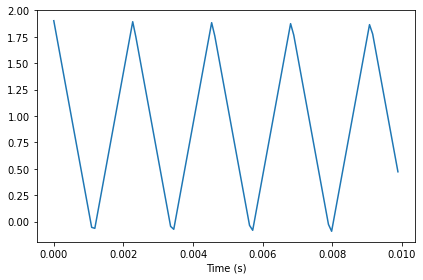
\includegraphics[scale=1]{fig/lab02/lab02_09.png}
		\caption{Обновленный график сигнала}
	\end{center}
\end{figure}

Получили смещение относительно вертикальной оси.


\subsection{Упражнение 4}

Напишите функцию, которая принимает Spectrum в качестве параметра и модифицирует его, деля каждый элемент hs на соответствующую частоту из fs. Протестируйте свою функцию, используя один из файлов WAV в репозитории или любой объект Wave.

1. Рассчитайте спектр и начертите его.

2. Измените спектр, используя свою функцию, и снова начертите его.

3. Сделать волну из модифицированного Spectrum и прослушать ее. Как эта операция влияет на сигнал?

Создадим функцию для деления spectrum.hs на соответствующую spectrum.fs

\begin{lstlisting}[language=Python]
def spec_div(sp):
  sp.hs[1:] /= sp.fs[1:]
  sp.hs[0] = 0
\end{lstlisting}

Проверим на пилообразном сигнале

\begin{lstlisting}[language=Python]
saw = SawtoothSignal()
saw_wave = saw.make_wave(duration=0.2, framerate=10000)
saw_wave.make_audio()

saw_sp = saw_wave.make_spectrum()
saw_sp.plot()
decorate(xlabel='Frequency (Hz)')
\end{lstlisting}

\begin{figure}[H]
	\begin{center}
		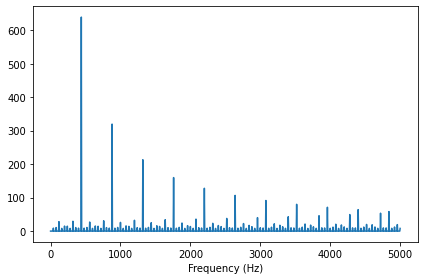
\includegraphics[scale=1]{fig/lab02/lab02_10.png}
		\caption{Спектр сигнала}
	\end{center}
\end{figure}

Применим функцию

\begin{lstlisting}[language=Python]
spec_div(saw_sp)
saw_sp.plot()
decorate(xlabel='Frequency (Hz)')
\end{lstlisting}

\begin{figure}[H]
	\begin{center}
		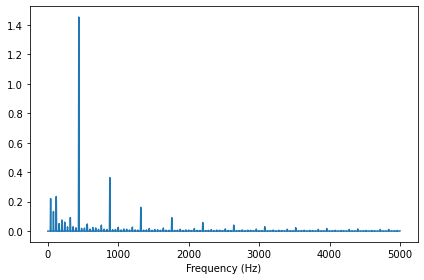
\includegraphics[scale=1]{fig/lab02/lab02_11.png}
		\caption{Спектр измененного сигнала}
	\end{center}
\end{figure}

\begin{lstlisting}[language=Python]
saw_sp.make_wave().make_audio()
\end{lstlisting}

Звук стал ниже


\subsection{Упражнение 5}

Треугольные и прямоугольные волны имеют только нечетные гармоники; пилообразная волна имеет как четные, так и нечетные гармоники. Гармоники прямоугольной и пилообразной волн затухают пропорционально $1/f$; гармоники треугольной волны затухают как $1/f^2$. Можете ли вы найти форму волны, в которой четные и нечетные гармоники затухают как $1/f^2$?

\noindent Подсказка: есть два способа подойти к этому: вы можете построить нужный сигнал путем сложения синусоид, или вы может начаться с сигнала, похожего на то, что вы хотите, и изменить его.

Создадим сигнал, который состоит из четных и нечетных гармоник, а также эти гармоники падают пропорционально квадрату частоты.

Возьмем пилообраный сигнал, так как у него четные и нечетные гармоники, надо его свести лишь к уменьшению гамони кропорционально квадрату

\begin{lstlisting}[language=Python]
saw = SawtoothSignal()
saw_wave = saw.make_wave(duration=0.5, framerate=20000)
saw_sp = saw_wave.make_spectrum()
saw_sp.plot()
decorate(xlabel='Frequency (Hz)')
\end{lstlisting}

\begin{figure}[H]
	\begin{center}
		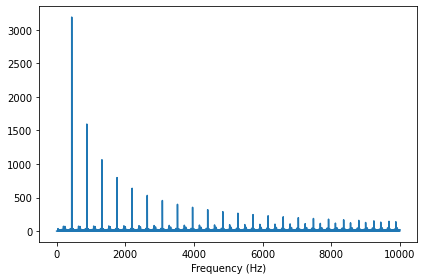
\includegraphics[scale=1]{fig/lab02/lab02_12.png}
		\caption{Спектр пилообразного сигнала}
	\end{center}
\end{figure}

Применяем функцию из прошлого упражнения

\begin{lstlisting}[language=Python]
spec_div(saw_sp)
saw_sp.plot()
decorate(xlabel='Frequency (Hz)')
\end{lstlisting}

\begin{figure}[H]
	\begin{center}
		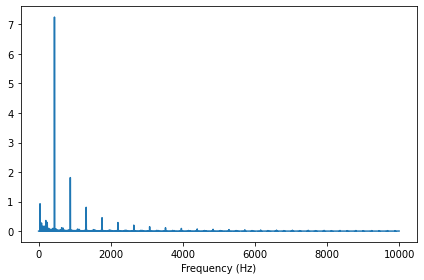
\includegraphics[scale=1]{fig/lab02/lab02_13.png}
		\caption{Спектр измененного сигнала}
	\end{center}
\end{figure}

Получаем, что амплитуда спадает пропорцинально квадрату частоты, имеются четные и нечетные гармоники.

\subsection{Вывод}

В данной работе были исследованы некоторые виды сигналов. Были рассмотрены спектры и гармонические структуры сигналов. Также в одном из пунктов были замечены биения и мы проверили их действие на звук.